%==========================================================================%
\documentclass[a4paper, 12pt]{article}

\usepackage{array}
\usepackage{amssymb}
\usepackage{times}
\usepackage[spanish, activeacute]{babel}
\usepackage{graphicx}
\usepackage{hyperref}
\usepackage[utf8]{inputenc}
\usepackage{fancyhdr}
\usepackage{xtab}
\usepackage{color}
\usepackage{lscape}
\usepackage{longtable}
\usepackage{tabularx}
%\usepackage{fontspec}
%\setsansfont{Gentium Basic}
\usepackage{colortbl}
\usepackage{graphics}
\usepackage{ltablex}
\usepackage{cite}
\usepackage{lscape}


\newenvironment{colortext}[1]{\color{#1}}{\ignorespacesafterend}

\renewcommand{\familydefault}{\sfdefault}




\hyphenation{de-ri-va-das} \hyphenation{le-bes-gue}
\hyphenation{e-llas} \hyphenation{o-cu-rrien-do}
\hyphenation{pro-pie-da-des}\hyphenation{pi-vo-te}
\hyphenation{dia-go-na-li} \hyphenation{e-cua-cion}
\hyphenation{a-pro-pia-dos}\hyphenation{ma-te-ma-ti-cos}\hyphenation{es-tu-dian-te}
\hyphenation{po-si-ti-vis-mo} \hyphenation{mo-de-li-za}





\pagestyle{fancyplain}

 \renewcommand{\sectionmark}[1]
                 {\markright{\thesection\ #1}}

 \newcommand{\coltex}[1]{\textcolor{red}{#1}}

                 
% \lhead[\fancyplain{}{\bfseries\thepage}]
%       {\fancyplain{}{\bfseries\rightmark}}
%
 \rhead[\fancyplain{}{\bfseries\leftmark}]{\fancyplain{}{\bfseries\thepage}}




 \lhead[\fancyplain{}{\vspace{-1cm}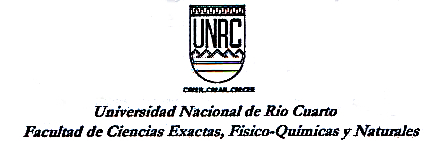
\includegraphics[scale=.4]{membrete.jpg}}]{\fancyplain{}{\vspace{-1cm}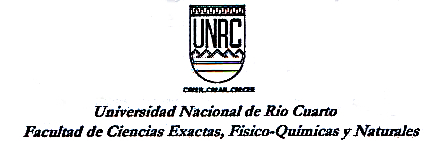
\includegraphics[scale=.4]{membrete.jpg}}}

\cfoot{}













\begin{document}

\title{PLAN DE ESTUDIOS DE LA CARRERA LICENCIATURA EN MATEMÁTICA}
\author{Plan 2022- Versión 0}
\date{}
 \maketitle

 \newpage



\tableofcontents

\newpage


\section{Identificación del proyecto}  

Plan de Estudios de la 
Carrera de Licenciatura en Matemática, de la Facultad de Ciencias Exactas, 
Físico - Químicas y Naturales, de la Universidad Nacional de Río Cuarto. Que reemplaza el Plan de Estudio de la Licenciatrura en Matemática aprobado por resolución del Consejo Directivo Nº 156/08, 
ratificada por resolución del Consejo Superior Nº 212/08.


\section{Responsables del proyecto}

\subsection{Unidad académica responsable de la elaboración del proyecto}

Comisión Curricular Permanente de la carrera Licenciatura en Matemática, dependiente de 
la Facultad de Ciencias Exactas Físico-Químicas y Naturales.

\subsection{Unidad académica responsable de la implementación del proyecto}

Facultad de Ciencias Exactas Físico-Químicas y Naturales. 



\section{Fundamentación}

\subsection{Razones que justifican la creación y o los cambios curriculares del proyecto de formación  y que justifican su realización}

La actualización  contenida en esta propuesta da cuenta de cambios en las normativas de la UNRC en cuanto a planes de estudio y a lineamientos para la elaboración de los  mismos. Más específicamente se trató de ajustar el Plan de Estudios de la Lic. en Matemática a:



\begin{enumerate}
 \item La Resolución CS-UNRC 297/2017 que aprobó el documento ``Hacia   un   currículo contextualizado, flexible e integrado. Lineamientos para la orientación de la innovación  curricular'' que define dimensiones que la Universidad considera importantes a la hora de elaborar planes de estudios, en particular dimensiones epistemólogico-metodológicas, de contextualización, organización, de flexibilidad e integración curricular. 

 \item La Resolución CS-UNRC 298/2017 que implementa el Proyecto de Innovación e Investigación para el Mejoramiento Estratégico Institucional (PIIMEI). Como parte de este Proyecto, la Comisión Curricular Permanente de la Licenciatura en Matemática junto con docentes y alumnos de la carrera emprendió una investigación del currículo de la carrera.  Parte de las conclusiones obtenidas fueron plasmandas en un Informe ``Actividades de Investigación Evaluativa
Licenciatura en Matemática'' el cual fue evaluado por expertos en curriculo universitario.

\item La Resolución CS-UNRC 510/2017 se actualizó el Plan Estratégico Institucional (PEI 2017-2023) el cual se constituye como documento orgánico con miras al desarrollo integral de la universidad, con emplazamiento geográfico y social. Los lineamientos del PEI de la UNRC representan la plataforma desde donde avanzar en la proyección de políticas institucionales de la Universidad en su conjunto y para nuestra Facultad en particular, que atienden necesidades actuales y proponen caminos de actuación a futuro.

\item La Resolución CD-FCEFQyN 410/2019 que aprueba el Plan Estratégico de la Facultad de Ciencias Exactas Físico-Químicas y Naturales (PEExa 2019-2023). En particular, en el Capítulo III, Sección 1 define objetivos de la institución para la enseñanza de grado.   

 \item La Resolución CS-UNRC 008/2021 que establece los conceptos, normas y procedimientos que regulan los procesos de elaboración, presentación, formalización, aprobación, seguimiento, evaluación y tramitación de reconocimiento de Nuevos Planes de Estudio y de modificaciones que impliquen nuevas versiones de los Planes de Estudio existentes.

\end{enumerate}

\subsection{Razones que determinan la conveniencia de la implementación de proyecto curricular  y que justifican su realización.}

La presente propuesta incorpora o profundiza los siguientes aspectos en la elaboración de planes de estudio: 

\begin{enumerate}
\item Contextualización y visión totalizante. Se analizaron las características de la población concreta de estudiantes a los que va dirigida la propuesta, las caracteríticas en cuanto a formación e intereses de investigación del plantel de docentes que ejecutará el plan, nuevas áreas emergentes, como el caso del análisis de grandes conjuntos de datos. Además se tomó en consideración aspectos administrativos, como por ejemplo aquellos que devienen del uso de la plataforma SIAL. 
\item Flexibilidad curricular. Al ciclo de optativas y trabajo final se agrega una materia electiva.
\item Organización curricular mixta. Se definen ciclos de formación y problemas transversales en la práctica docente. 
\item Transversalidad de la práctica profesional. Este punto es consecuencia del anterior.
\item Incorporación de espacios de formación socio-política-cultural con la incorporación de \textcolor{red}{xxxxxx}
\end{enumerate}

A esto se suma la necesidad de resolver las siguientes cuestiones más coyunturales del plan vigente.

\begin{enumerate}
\item Inconsistencia de la carga horaria de asignaturas homólogas en distintos planes de estudios (Probabilidades 1987).

\item Se modifican correlatividades atendiendo a necesidades emergentes de nuevos desafíos en la enseñanza (Probabilidades 1987). 

\item Mayor flexibilidad del ciclo de especialización. No se especifican materias optativas, en cuanto a contenidos ni siquiera nombres. Se detectó que en los planes previos la existencia de diversas materias optativas con diferentes denominaciones causaba problemas en cuanto a la ejecución del plan a nivel administrativo.  
\end{enumerate}


\subsection{Correspondencia con los fines y objetivos de la Universidad}

Los fines y objetivos de la Universidad y de la Facultad de Ciencias, Exáctas Físico-Químicas y Naturales están definidos en el Estatuto Universitario y en el Plan Estratégico Institucional (PEI) y en el Plan Estratégico  de la Facultad (PEExa). El plan de estudios de la Licenciatura de Matemática se enmarca dentro de los objetivos y fines declarados en los anteriores documentos, especialmente por las consideraciones en ellos establecidas  que enumeramos debajo. 


\begin{description}
 \item[Estatuto de la UNRC.]   Aprobado por Resolución Ministerio de Educación Nº1723/2011.  Se define que la Universidad es:
\begin{enumerate}

\item ``Productora, distribuidora y difusora de conocimiento socialmente útil y público, es
decir, provisional, histórico, criticable, no dogmático, hipotético, abierto a la
pregunta, al cuestionamiento y al contraste riguroso. Como tal deberá ser reflexiva
y proactiva, capaz de autoevaluarse en forma permanente y, así, comprender y
mejorar sus procesos y sus productos''


\item ``Una institución que busca la excelencia académica al ofrecer a los estudiantes
conocimientos y prácticas de máxima calidad y de significación científica y social''

\item ``Flexible para adaptarse a la diversificación y expansión de la población estudiantil, 
a las nuevas tecnologías, a las formas de comunicación y producción de
conocimiento, a la movilidad de las profesiones, a la evolución de los paradigmas
de la ciencias y a las nuevas condiciones sociales.''

\item ``Innovadora en sus formas de enseñanza, investigación y transferencia educativa y
tecnológica''

\item ``Una institución articulada con el nivel medio, con el subsistema de educación
superior no universitaria, con otras Universidades de la región, del país y del
mundo y con otras organizaciones sociales y por tener la capacidad de dar
respuestas contextualizadas con lo regional''

\end{enumerate}

\item[PEI 2017-2023] Se definen como Ejes Estratégicos prioritarios en la agenda universitaria:
\begin{enumerate}
 \item Inclusión    educativa    con    calidad    para         todos  los  estudiantes  de  la  universidad  pública.
 
 \item  Actualización  y  flexibilidad  del  currículo  en la enseñanza de grado y posgrado.
 
 \item Producción  de  conocimiento  científico,  técnico y artístico con alto nivel y sentido social. 
\end{enumerate}

\item[PEExa 2019-2023] Define como objetivos de la enseñanza de grado:
\begin{enumerate}
 \item  La actualización curricular.
 \item Sostenimiento y fortalecimiento de la formación integral.
\item Orientación de los procesos de enseñanza y de aprendizaje hacia el
conocimiento de la realidad local, nacional e internacional.
\item Fortalecimiento de modalidades de enseñanza con TICs.
\item Mejoramiento de las prácticas y formación docente.

\end{enumerate}

\end{description}

Por otra parte los objetivos de este plan de estudios están en correspondencia con:

\begin{description}
\item[Prioridades de Investigación de la UNRC] Definidas en la Resolución CS-UNRC 302/2018. 
En ella se consignan las áreas y temas de interés, en particular las área 8 de Matemática y Computación.
\item[Líneas curriculares para la UNRC] Descriptas en las Resoluciones CS-UNRC 297/2017 y 008/2021.
\end{description}




\subsection{Antecedentes}

\subsubsection{Breve reseña del origen y trayectoria de la carrera, considerando los ámbitos nacional, regional e institucional.}

 La enseñanza de la matemática en territorio argentino se remonta a la  época colonial. Instaurado el primer gobierno patrio,  Manuel Belgrano fue un impulsor del estudio de las ciencias con  la creación de la   Escuela de Matemáticas  el 12 de setiembre de 1810 (ver \cite{stacco2011200}). 

 Una de las primeras menciones que hemos hallado de una carrera denominada Licenciatura en Matemática es en  \cite{ortiz2011julio} 
 donde se menciona que en  1926 se creo una Licenciatura y un Doctorado en Matemática y en Física dentro de una Facultad de Ingeniería. 

 Posteriormente el estudio de la matemática superior se ha diseminado por todo el sistema de educación superior Argentino, siendo una de las carreras con más larga trayectoria en el país. En la actualidad la carrera de Licenciatura en Matemática se ofrece en las siguientes universidades nacionales: UNRC, UNAB, UNSL, UNC, UNLPam, UNNE, UNICEN, UNL, UNCOMA, UNMDP, UNSJB, UNS, UNSE, UNR y UBA.  
 
 En la UNRC la carrera de Lic. en Matemática fue creada desde el origen de la universidad. Su primer plan de estudios fue aprobado por Resolución Ministerial  N° 1560/80 en el año 1975. Consistió en una carrera de 5 años de duración Posteriormente el plan fue modificado en 1993, 2001 y 2008. El plan de 1993 incorporó como una de sus características centrales la elaboración de un trabajo final. Además se introdujeron cambios en pos de articular con las carreras de computación recientemente creadas.  En el plan de 2001 se revierten en parte los cambios anteriores, separando algunas  materias respecto a las correspondientes de las carreras de  computación y se introducen cambios en las áreas de geometría y estadística.  
 El plan de  2008 llevó a la carrera a 4 años. Entre los aspectos centrales contenidos en este plan citamos que se hizo explícito el objetivo de incorporar la formación interdisciplinaria. La implementación del mismo obedeció en parte a recomendaciones elaboradas por la Unión Matemática Argentina en su documento \cite{uma}.  Fue aprobado por Resolución del CD-FCEFQyN Nº 258 /07, ratificada 
por Resolución del CS-UNRC Nº 289/07. Registro y toma de conocimiento 
por parte de la Dirección Nacional de Gestión Universitaria informado por nota 
Nº 544/08. Introducción de modificaciones, que generaron la versión 1 del Plan 
de Estudios, aprobadas por resolución del CD-FCEFQyN Nº 156/08, 
ratificada por resolución del CS-UNRC Nº 212/08.  Nueva introducción de modificaciones, que generaron la versión 2 aprobada por Resolución del CD-FCEFQyN N° 340/17, por la cual se aprueba el Texto Ordenado del Plan de Estudios 2008, Versión 2, de la Carrera de "Licenciatura en Matemática", según consta en el Anexo 1 de la citada Resolución, obrante a fojas 180/216 del Expediente N° 88664.  Resolución del CS-UNRC N° 443/17, por la cual se ratifica la Resolución  CD-FCEFQyN N° 340/17.  La versión 2 del Plan 2008 aún no se encuentra vigente. 




\subsubsection{Actividades de docencia, investigación o extensión realizadas por la universidad vinculadas  al proyecto.}

\begin{description}
 \item[Docencia] Como se mencionó hay una larga trayectoria  de nuestra Facultad en el dictado de carreras de grado y posgrado  vinculadas con la matemática, particularmente la Licenciatura en Matemática, el Profesorado en Matemática, Maestría en Matemática Aplicada y Especialidad en Didáctica de la Matemática. Además de estos antecedentes, merece mencionarse que diversas carreras de nuestra y de otras facultades requieren el dictado de materias vinculadas con la matemática y por tanto es necesario la formación de docentes altamente calificados en esta disciplina. Nuestros egresados forman parte de los departamentos de matemática de otras facultades de nuestra universidad.
 
 \item[Investigación] Dentro del departamento de matemática de la FCEFQyN se ejecutan regularmente  proyectos financiados tanto por SECyT-UNRC como por organismos de financiamiento de actividades científicas de orden  nacional como ANPCyT y CONICET. Investigadores y becarios del CONICET desarrollan sus actividades en la mencionada unidad académica. Se participa de proyectos y grupos interdisciplinarios, por ejemplo en  facultades de ingeniería, miembros del departamento forman parte  del Instituto de Investigaciones Sociales, Territoriales y  Educativas. Por otra parte se desarrollan actividades de investigación que requieren fuertemente el uso de la matemática en otras facultades de nuestra universidad, por ejemplo en las Facultades de Ciencias Económicas (FCE) e Ingeniería (FI).
 

 
 
\end{description}






\subsubsection{Experiencias similares realizadas a nivel nacional o internacional que hubieran sido tenidas en cuenta.}

En la elaboración de este plan de estudios se tuvieran en cuenta las siguientes experiencias y antecedentes.
\begin{description}
 \item[Unión Matemática Argentina]  Es la asociación que agrupa a los matemáticos del país.  La UMA convocó a matemáticos de reconicida trayectoria a nivel internacional, quienes elaboraron un documento (ver \cite{uma}) 
 dando cuenta de sugerencias curriculares para la carrera de Licenciatura en Matemática.
 
 \item[Foro UMA-CUCEN] En el marco de las reuniones periódicas del Consejo Universitario Ciencias Exactas y Naturales (CUCEN) se realizó durante los años 2017-2018 un foro donde se debatieron ciclos de formación con el propósito de favorecer la movilidad de los estudiantes entre carreras de Licenciatura en Matemática del país. Nuestra carrera participó activamente de este foro. Es de destacar que fruto de esta participación, y como parte del proyecto PIIMEI, se hizo una comparativa entre los distintos planes, más específicamente se definieron distintas nudos conceptuales y se identificaron las carreras de Licenciatura en Matemática de Argentina que trabajan dichos nudos (ver \cite{CCP}). 

\item[Sistema Nacional de Reconocimiento Académico (SNRA)] Fue creado por la Resolución Ministerial N° 1870/16. Es un sistema voluntario de acuerdos entre instituciones de Educación Superior de la Argentina, que permite el reconocimiento de trayectos formativos (tramos curriculares, ciclos, prácticas, asignaturas, materias u otras experiencias formativas) para que los estudiantes transiten por el sistema aprovechando toda su diversidad y profundizando la experiencia de formación.

En el marco del SNRA el Ministerio de Educación convocó a especialistas de todo el sistema de educación superior, incluído doncentes de nuestra Licenciatura en Matemática,  para que definan trayectos formativos con el propósito de facilitar la movilidad estudiantil dentro del sistema de ecucación superior nacional. 

Fruto de la participación antes aludida nuestra universidad suscribió convenios de reconocimiento de trayectos académicos dentro del área matemática. Este plan de estudio refleja los acuerdos expresados dentro de estos convenios.

\item[Proyecto Tuning] Tuning es una red de comunidades de aprendizaje de alcance internacional, integrada por académicos y estudiantes interconectados, que reflexiona, debate, elabora instrumentos
y comparte resultados. Siguiendo a \cite{paniagua2013educacion},
 ``Tuning es una metodología con pasos bien diseñados, y una perspectiva dinámica que permite la adaptación a los diferentes contextos. La metodología tiene un objetivo claro: construir titulaciones compatibles, comparables, relevantes para la sociedad y con niveles
de calidad y excelencia, preservando la valiosa diversidad que viene de las
tradiciones de cada uno de los países.'' 

Para el diseño de la presente propuesta curricular se tuvo en consideración el documento \cite{paniagua2013educacion} 
que estudia perfiles del egresado y escenarios de futuro para el Área de Matemática y la profesión y estrategias de enseñanza, aprendizaje y evaluación de las competencias propias de los profesionales del área. 

\item[Competencias matemáticas para la industria] 
Es una preocupación permanente en el diseño del plan de estudios de la Licenciatura en Matemática, tanto en esta institución como otras, la inserción del egresado en ámbitos no académicos. Generalmente  en la bibliografía se refiere a estos ámbitos como la ``industria'',  se contempla que estos incluyen organismos públicos, empresas informáticas, etc. Diversas organizaciones se han encargado de identificar aquellas competencias que son requeridas en industrias a profesionales y que pueden ser provistas por egresados del área de las matemáticas y han propuesto estrategias pedagógicas para la consecución de estas competencias. Hemos estudiado los siguientes antecedentes en esta materia.

La Society for Industrial and Applied Mathematics (SIAM)  es una asociación académica dedicada al uso de las matemáticas en la industria que tiene conexiones con la Asociación Argentina de Matemática Aplicada Computacional e Industrial. La SIAM publicó varios documentos sobre la problemática del matemático en la industria, en particular \cite{society1996siam,society2012siam}.


 La Comisión Internacional de Instrucción Matemática (ICMI) es una comisión de la Unión Internacional de Matemáticas (IMU) y es una organización de actuación internacional centrada en la educación matemática. La ICMI publicó las Educational Interfaces between Mathematics and Industry (ver \cite{damlamian2013educational}) entre otros materiales dirigidos a la temática en cuestión.
\end{description}



\subsubsection{Población destinataria}

La población destinataria de la carrera es la definida por la Resolución CS-UNRC 120/2017 que aprobó el ``Régimen  de estudiantes y de enseñanza de pregrado y grado de la UNRC''. En el punto 2 del Anexo I de la mencionada normativa se establecen las condiciones para que un estudiante ingrese a una carrera de grado dentro del ámbito de la UNRC.




\subsubsection{Rasgos y características de la población estudiantil que atiende: tener en cuenta los destinatarios reales y potenciales de la formación, considerando las condiciones y cualidades sociales, culturales y económicas que la caracterizan en general y según los grupos de procedencia: diversidades culturales, mayores de 25 años sin título secundario, culturas juveniles vigentes y emergentes, personas en situación de discapacidad, adultos mayores, estudiantes de pueblos originarios, de diferentes lugares del país y extranjeros, entre otros.}

\textcolor{red}{Cómo caracterizaríamos nuestros estudiantes? SINTETIZAR  ARCHIVO COMPARTIDO POR MARCELO}

\section{Objetivos del proyecto}


Formar un egresado:

\begin{enumerate}

 \item Con capacidad crítica y autocrítica,
 \item Respetuoso de los valores democrácticos y de la diversidad cultural,  
  \item Con un alto conocimiento técnico en la disciplina,
 \item Capacitado en la aplicación de la matemática en la
resolución de problemas científicos y/o tecnológicos,
\item Que pueda acceder a carreras de posgrado.
nacionales y del extranjero, 
\item Capaz de integrarse en grupos de trabajo interdisciplinarios,
\item Capaz de plantear y resolver problemas de matemática pura,
\item Alentar al estudiante para que tome contacto con problemas de
    investigación en distintos momentos de la carrera por medio de espacios extracurriculares destinados a este fin.
\end{enumerate}







\section{Características de la carrera}


\subsection{Nivel} Carrera de grado.

\subsection{Acreditación} Licenciado en Matemática.

\subsection{Alcance del título} Esta carrera habilita para:
\hyphenation{de-sa-rro-llo}
    \begin{enumerate}

        \item Participar en equipos interdisciplinarios que utilicen la matemática.
        
        \item  Realizar actividades de investigación en proyectos de matemática         pura o aplicada.
       
       \item Intervenir  como peritos matemáticos en  organismos públicos o privados  tales como, INDEC,  empresas que realicen desarrollos tecnológicos, bancos,   compañías de seguro, etc.
       
        \item Acceder a carreras de posgrado.
       
       \item Participar de los equipos docentes dirigidos a la
         enseñanza de la matemática en los niveles superiores de enseñanza.
    
       
         
    \end{enumerate}

\subsection{Actividades profesionales reservadas al título (Incumbencias)}
    
\subsection{Perfil del Título}
 


\subsubsection{Conocimientos que constituyen el fundamento teórico-metodológico de su accionar profesional o académico.}

Se aspira a que el Lic. en Matemática adquiera un conocimiento sólido en las siguientes  áreas de
 la matemática: Análisis Matemático, Funciones de una Variable Compleja,   Teoría de la Medida, Probabilidades. Estadística. Ciencia de Datos, Geometría Diferencial, Álgebra Lineal, Estructuras Algebracicas, Ecuaciones Diferenciales ordinarias y parciales, Cálculo Numérico, Análisis Funcional.
 
 Se pretende además que el estudiante adquiera conceptos básicos de programación, mecánica y en una materia proveniente de otra ciencia, por ejemplo biología, economía, química, física, ingeniería, informática. Para esto último se prevé una  materia electiva. 

 Se aspira además a que el estudiante logre una formación complementaria en un área de su elección dentro de la oferta de que disponga como parte de su ciclo de especialización.
 
\subsubsection{Capacidades y habilidades requeridas para la realización de las actividades que le incumben.}


Se espera lograr un profesional capacitado para:
\begin{enumerate}

\item { Actuar con responsabilidad social y compromiso
ciudadano,} 



\item {Aprender, actualizarse y trabajar de manera autónoma,} 
 


\item {Realizar análisis  críticos y autocríticos,} 
 
\item {Plantear y resolver problemas de matemática pura,} 

\item{Idear demostraciones,}

\item {Valorar y respetar  la diversidad
y la multiculturalidad,} 
 




 

\item {Construir y desarrollar
argumentaciones lógicas con una
identificación clara de hipótesis y conclusiones,} 
 
\item {La abstracción (extraer de una situación los rasgos más relevantes),} 
 


\item {Formular problemas
en lenguaje matemático,} 
 

  


\item {Iniciar investigaciones
matemáticas bajo orientación de experto,} 
 


 
 


\item {Contribuir en la
construcción de modelos matemáticos a
partir de situaciones reales,} 
 


\item {Utilizar las herramientas
computacionales de cálculo numérico
y simbólico para plantear y resolver
problemas,} 
 


\item {Analizar  grandes conjuntos de datos,} 
 


\item {Expresarse correctamente
utilizando el lenguaje de la
matemática,} 
 


\item {Comunicarse
con otros profesionales no matemáticos,} 

 

\item {Actuar en contextos educativos y planificar actividades de enseñanza,} 
 


\item {Leer, escribir y exponer documentos en
inglés, así como comunicarse con otros
especialistas,} 

 


\item {Trabajar en equipos
interdisciplinarios.} 

\end{enumerate}


\subsection{Requisitos de ingreso}



Los fijados por el ``Régimen  de estudiantes y de enseñanza de pregrado y grado de la UNRC'', ver  el punto 2 del Anexo I de la Res. CS. 120/2017. 



\subsection{Organización del Plan de Estudios}

\subsubsection{Ciclos, Trayectos  y Áreas} El Plan de Estudios se desarrollará en tres ciclos:
un ciclo básico común con el profesorado, un ciclo superior y un
ciclo de especialización.

\paragraph{Ciclo Básico} El ciclo básico incluye 11 asignaturas.

\setlength\arrayrulewidth{1pt}
\begin{center}
\begin{tabularx}{1\textwidth}{|>{\raggedleft\arraybackslash}X |
>{\raggedleft\arraybackslash}X |
>{\raggedleft\arraybackslash}X |
>{\raggedleft\arraybackslash}X |}
\hline
  \rowcolor[gray]{.9}
  \emph{Asignaturas del ciclo básico} & Código  & \emph{Horas semanales} &  \emph{Horas totales}
  \\\hline
  Cálculo I                          &   1921   &           8   &   112          \\ \hline
  Matemática Discreta       	     &   1925   &           8   &   112          \\ \hline
  Geometría I               	     &   1935   &           6   &    84          \\ \hline
  Cálculo II                         &   1928   &           8   &   112          \\ \hline
  Álgebra Lineal I                   &   1933   &           8   &   112          \\ \hline
  Taller de informática              &   1927   &           6   &    84          \\ \hline
  Cálculo III                        &   1929   &           8   &   112          \\ \hline
  Probabilidades                     &   1987   &           8   &   112          \\ \hline
  Estructuras Algebraicas            &   1993   &           8   &   112          \\ \hline
   Estadística                        &   1991   &           6   &    84          \\ \hline
  Física                             &   1930   &           6   &    84          \\ \hline
  \emph{Total de horas ciclo básico }& \multicolumn{3}{r|}{\emph{1136}}            \\ \hline
\end{tabularx}
\end{center}


\paragraph{Ciclo Superior} Consta de 13 materias
obligatorias.

\begin{center}
\begin{tabularx}{1\textwidth}{|>{\raggedleft\arraybackslash}X |
>{\raggedleft\arraybackslash}X |
>{\raggedleft\arraybackslash}X |
>{\raggedleft\arraybackslash}X |}
\hline
  \rowcolor[gray]{.9}
\emph{Asignaturas del ciclo superior  }  & Código &\emph{Horas semanales} &  \emph{Horas totales}\\ \hline
Inglés  (Anual)                            & 1976   &           4        &     112          \\ \hline
Estudio de la Realidad Nacional          & 6235   &           2        &      28           \\ \hline
Cálculo Numérico  Computacional          & 2030   &           8        &     112           \\ \hline
Topología                                & 1917   &           8        &     112           \\ \hline
Álgebra Lineal Aplicada                  & 2261   &           8        &     112           \\ \hline
Fundamentos de Análisis           &   xxxx &             8        &             112    \\ \hline
Variables Complejas   & 1911   &           8        &     112           \\ \hline
Medida e Integración                     & 2263   &           8        &     140           \\ \hline
Ecuaciones Diferenciales                 & 1913   &           8        &     112           \\ \hline
Geometría Diferencial                    & 1915   &           8        &     112           \\ \hline
Modelos de regresión y metodos empíricos  & XXXX  &           6 
& 90   \\ \hline
Introducción a las Ecuaciones en Derivadas Parciales &   2212  & 8 & 112  \\ \hline
Análisis Funcional               &    1916   &       8        &            112      \\ \hline
\emph{Total de horas ciclo superior }    &\multicolumn{3}{r|}{\emph{1322 }}                    \\ \hline

\end{tabularx}
\end{center}



\paragraph{Ciclo de Especialización} Dirigido a introducir al alumno
en la investigación en una rama específica de la matemática de su elección o a introducirlo en las aplicación de la matemática a un problema de modelización o aplicación de la matemática a un problema de origen tecnológico, social, productivo, etc. 

Consta de dos asignaturas optativas una electiva y contempla la realización de un trabajo final. La realización del trabajo final está regulado por la Res. CD. FCEFQyN N0 208/91 o aquella que la suplante.    

\begin{center}
\begin{tabularx}{1\textwidth}{|>{\raggedleft\arraybackslash}X |
>{\raggedleft\arraybackslash}X |
>{\raggedleft\arraybackslash}X |
>{\raggedleft\arraybackslash}X |}
\hline
  \rowcolor[gray]{.9}
\emph{Asignaturas del ciclo de especialización  } & Código&\emph{Horas semanales} & 
\emph{Horas totales}      \\ \hline
Optativa I                     &           &            8        &         112        \\ \hline
 Electiva                 &            &    6                &        84          \\ \hline
 Optativa II                    &            &           10         &          140        \\ \hline
 Trabajo Final                     & 2265         &       10             &          140        \\ \hline
\emph{Total de horas ciclo de especialización}    & \multicolumn{3}{r|}{\emph{476 }} \\ \hline
\end{tabularx}
\end{center}



\subsubsection{Listado total de asignaturas}
\fontsize{10pt}{10pt}\selectfont  
\begin{center}

\begin{tabularx}{1\textwidth}{|>{\raggedleft\arraybackslash}X |
>{\raggedleft\arraybackslash}X |
>{\raggedleft\arraybackslash}X |
>{\raggedleft\arraybackslash}X |
>{\raggedleft\arraybackslash}X |}
\hline
\hline
\rowcolor[gray]{.9}\multicolumn{5}{|c|}{\textbf{Primer año}}                                                        \\ \hline

\emph{Cuat. }  &\emph{Código}  & \emph{Materia}                              &    hr. sem.       &  hr. Tot.        \\ \hline

I              & 1921          & Cálculo I                                &          8  &   112     \\ \hline
I              & 1925          & Matemática Discreta                      &          8  &   112       \\ \hline
I              & 1935          & Geometría I                              &          6  &    84       \\ \hline
\multicolumn{3}{|l|}{\textbf{Total de Horas cuatrimestre I}}              &\textbf{22 } &\textbf{308 }\\ \hline
II             & 1928          & Cálculo II                               &          8  &   112       \\ \hline
II             & 1933          & Álgebra Lineal I                         &          8  &   112       \\ \hline
II             & 1927          & Taller de informática                    &          6  &    84       \\ \hline
\multicolumn{3}{|l|}{\textbf{Total de Horas cuatrimestre II}}             &\textbf{22 } &\textbf{308 }\\ \hline
 
\rowcolor[gray]{.9}
\multicolumn{5}{|c|}{\textbf{Segundo año}}                                                                \\ \hline
III            & 1929          & Cálculo III                              &          8  &   112      \\ \hline
III            & 2030          & Cálculo Numérico  Computacional          &          8  &   112    \\ \hline
III            & 1976          & Inglés (Anual)                           &          4  &    56     \\ \hline
III            & 2064          & Sociología de la Educación                           &          4  &    56     \\ \hline
\multicolumn{3}{|l|}{\textbf{Total de Horas cuatrimestre III}}            & \textbf{24 }&\textbf{336 }\\ \hline
IV             & 1987          & Probabilidades                           &          8  &   112      \\ \hline
IV             & 1993          & Estructuras Algebraicas                  &          8  &   112      \\ \hline
IV    &  1976 & Inglés (Anual) & 4  & 56 \\ \hline
\multicolumn{3}{|l|}{\textbf{Total de Horas cuatrimestre IV}}             &\textbf{20 } &\textbf{280 }\\ \hline

\rowcolor[gray]{.9}\multicolumn{5}{|c|}{\textbf{Tercer año}}                                                        \\ \hline
V              & 1991          & Estadística                                &           6         &         84         \\ \hline
V              & XXXX          & Fundamentos de Análisis           &            8        &             112     \\ \hline
V             & 2261          & Álgebra Lineal Aplicada                  &          8  &   112       \\ \hline

\multicolumn{3}{|l|}{\textbf{Total de Horas cuatrimestre V}}                &\textbf{22}           &\textbf{308}         \\ \hline
VI             & 1930          & Física                                     &            6        &           84       \\ \hline
VI             & 1911          & Variables Complejas                          &             8       &         112         \\ \hline
VI             & 6235          & Estudio de la Realidad Nacional *          &               2     &         28         \\ \hline
VI            & 1917          & Topología                                   &              8      &        112          \\ \hline
\multicolumn{3}{|l|}{\textbf{Total de Horas cuatrimestre VI} }              &\textbf{24}           &\textbf{336}         \\ \hline
  
\rowcolor[gray]{.9}\multicolumn{5}{|c|}{\textbf{Cuarto año}}                                                        \\ \hline
VII           & 2263          & Medida e Integración                       &             10       &            140     \\ \hline
VII            & 1913          & Ecuaciones Diferenciales                   &           8         &        112          \\ \hline
\multicolumn{3}{|l|}{\textbf{Total de Horas cuatrimestre VII}}              & \textbf{18}          &\textbf{252}         \\ \hline
VIII             & 1915          & Geometría Diferencial                      &              8     &        112          \\ \hline
VIII           & xxx           & Modelos de regresión y metodos empíricos                  &              6      &         84         \\ \hline

% VIII           & 2265          & Modelos Matemáticos                        &               6     &       84           \\ \hline

VIII          & 2212           & Introducción a las Ecuaciones en Derivadas Parciales & 8  & 112  \\ \hline

\multicolumn{3}{|l|}{\textbf{Total de Horas cuatrimestre VIII}}             & \textbf{22}          &\textbf{308}         \\ \hline

\rowcolor[gray]{.9}\multicolumn{5}{|c|}{\textbf{Quinto año}}                                                        \\ \hline
IX            &  1916         &  Análisis Funcional               &           10         &            140     \\ \hline
IX           &               & Optativa I                                &            8        &         112        \\ \hline
X           &           & Electiva                             &    6                &        84          \\ \hline
\multicolumn{3}{|l|}{\textbf{Total de Horas cuatrimestre VII}}              & \textbf{24}          &\textbf{336}         \\ \hline
X           &               & Optativa II                                &           10         &          140        \\ \hline
X           & 2265          & Trabajo Final                              &       10             &          140        \\ \hline


\multicolumn{3}{|l|}{\textbf{Total de Horas cuatrimestre VIII}}             & \textbf{20}          &\textbf{280}         \\ \hline
\multicolumn{4}{|l|}{\textbf{Total de Horas del Plan de estudios}}                               &\textbf{}         \\ \hline
\end{tabularx}
\end{center}
\normalsize



\subsubsection{Contenidos y metodología}
\paragraph{Contenidos}
\subparagraph{Ciclo Básico}

\begin{enumerate}

\item \textbf{Cálculo I (1921):} Números Reales. Funciones
trascendentes. Operaciones con funciones. Límite. Continuidad.
Derivadas. Aplicaciones de la Derivada: máximos, mínimos, trazado
de curvas. Teorema del valor medio: Aplicaciones.

Bibliografía Principal: \cite{PeterD.Lax631}.

Bibliografía Consulta: \cite{MichaelSpivak649}

Bibliografía orientada por la historia: \cite{ErnstHairer633,DavidApplebaum639,OttoToeplitz642,DavidBressoud643,DavidM.Bressoud651,DavidM.Bressoud688}.


 
\item \textbf{Matemática discreta (1925):} Introducción a la lógica. Números
naturales. Principio de inducción. Introducción a la combinatoria.
Números enteros: Divi\-sibilidad, Teorema fundamental de la
Aritmética, Congruencia,  Ecuaciones Diofánticas, Teorema de
Fermat y Euler. Relaciones y funciones: funciones inyectivas,
suprayectivas, relaciones de orden y de equivalencia.

Bibliografía Principal: \cite{gentile, grimaldi}.




\item \textbf{Geometría I (1935):} Triángulos: medianas, mediatrices, centroides. Inscriptos y
circunscriptos. Ortocentro. Polígonos: simetrías. Isometrías del
plano euclídeo. Geometría afín: ecuaciones de rectas  en
el plano y de rectas y planos en el espacio. Espacios vectoriales generales.
Transformaciones lineales: rotaciones, reflexiones, simetrías.
Cónicas y cuádricas.
Bibliografía Principal: \cite{AllanBerele41,RogerFenn248,RobinHartshorne131,AlfredS.Posamentier49}.

Bibliografía de Consulta: \cite{O.Bottema149,CharlesStanleyOgilvy129,AllanBerele41,GerardA.Venema145,H.S.M.Coxeter226,H.S.M.Coxeter35,MatthewHarvey261,RogerA.Johnson42,coxeter,GJE,villamayor}.




\item \textbf{Cálculo II (1928):}   Integral definida de una variable real: áreas, volúmenes,
longitudes, etc. Métodos de integración, integrales impropias.
Sucesiones y series numéricas. Series de potencias. Series de
Taylor. Introducción a las  ecuaciones diferenciales de primer
orden.


Bibliografía Principal: \cite{PeterD.Lax631,GeorgeFinlaySimmons487}.

Bibliografía Consulta: \cite{MichaelSpivak649,ErnstHairer633,DavidApplebaum639,OttoToeplitz642,DavidBressoud643,DavidM.Bressoud651,DavidM.Bressoud688}.





\item \textbf{Taller de Informática (1927).} Noción de algoritmo. Su formulación en pseudocódigos. Estructuras de datos y de control. Implementación
en lenguaje computacional.

Bibliografía sugerida: \cite{Seroul:2000,Rose:2015}.




\item \textbf{Álgebra Lineal I (1933):} Espacios vectoriales. Transformaciones
lineales y matrices. Teorema de la dimensión. Rango de una matriz.
Espacio dual. Espacio euclídeo. Bases ortonormales. Polinomios.
Autovalores y autovectores. Dia\-gonalización.

Bibliografía sugerida: \cite{hoffman, strang}.


\item \textbf{Cálculo III (1929):} Funciones vectoriales. Derivadas. Longitud de
arco. Funciones de varias variables. Derivadas parciales. Regla de
la cadena. Derivadas direccionales. Extremos y extremos
condicionales. Integración múltiple. Aná\-lisis vectorial.
Integrales de línea y de superficie. Teoremas de Green, Gauss y
Stokes.

Bibliografía sugerida: \cite{ marsdentromba,MarianoGiaquinta641,ErnstHairer633,PeterD.Lax632}.




\item\textbf{Inglés (1976):} Inglés nivel básico: Verbos \emph{to be}, \emph{to
have}. Uso de \emph{some} y \emph{any}. El presente simple. El
pasado simple. Uso de little, \emph{few, much, many, each, either,
every, both}. La voz pasiva. La forma \emph{ing}. El infinitivo.
Expresiones de comparación. Formas superlativas. Sentencias
condicionales. Futuro simple.  Análisis de textos relacionados con la
ciencia matemática; enfatizando el reconocimiento de: elementos no
ling\"{u}ísticos, elementos ling\"{u}ísticos ( nivel: léxico,
sintético, morfológico y semántico) y funciones del lenguaje
(descripción, definición, clasificación, etc.).



\item \textbf{Probabilidades (1987):} Espacios de probabilidad.  Probabilidad
condicional e independencia.  Variables aleatorias y sus distribuciones.  Vectores aleatorios y transformaciones.  Dependencia y distribuciones condicionales. Función generatriz de momentos y sus aplicaciones. Convergencia de variables aleatorias. Ley débil y ley fuerte de
los grandes números. Teorema Central del Límite. 

Bibliografía sugerida: \cite{berts, parzen, ross, grimmet}. 

\item \textbf{Estructuras Algebraicas  (1993):} Grupos. Grupos cíclicos y
simétrico. Acción de un grupo en un conjunto. Teoremas de Sylow.
Anillo. Dominios Euclidianos, Principales y de Factorización
única. Módulo. Módulos: Finitamente Generados, Libres.
Divisibilidad.

Bibliografía sugerida: \cite{ gentile,herstein, lang}.



\item\textbf{Álgebra Lineal Aplicada (2261):}  Normas matriciales.
Método de Gram-Schmidt. Descomposición QR.
Matrices unitarias y ortogonales. Reducción ortogonal.
Descomposición SVD. Diagonalización. Matrices normales y simétricas. Matrices
definidas positivas. Matrices nilpotentes y formas de Jordan.

 Bibliografía sugerida: \cite{golub,hoffman,meyer, strang}


 \item \textbf{Estadística (1991):} Estadística Descriptiva. Distribuciones de muestreo. Estimación Puntual. Intervalos y Regiones de Confianza. Pruebas de Hipótesis. Pruebas de $\chi$-Cuadrado. Modelos de regresión lineal. Métodos empíricos. 

Bibliografía sugerida: \cite{wasserman, devore, witten, boente, mosche}
 
\item \textbf{Fundamentos de análisis:} Cardinalidad. Espacios métricos. Completitud. Conexión. Compacidad. Convergencia uniforme. $M$-test Weiertrass. Series de potencias y de Fourier. Convergencia uniforme y su relación con la continuidad, la  derivada y la  integral. Teorema punto fijo de Banach. Aplicación: Teorema de Existencia y Unicidad de soluciones ecuaciones diferenciales ordinarias.  
Bibliografía sugerida: \cite{RogerGodement658,StephenAbbott134,Simmons671,MichealOSearcoid674,SatishShirali675,VictorBryant676,J.Dieudonne678,WalterRudin681,NikolaosKatzourakis684,VilmosKomornik685,VicenteMontesinos686}











\item\textbf{Física (1930):} Mecánica. Dinámica de una partícula. Leyes
de Newton. Concepto de masa. Energía cinética y potencial. Fuerzas
de vínculo. Fuerza centrípeta. Fuerzas de rozamiento. Ley de
gravitación universal. Ecuaciones de movimiento. Momentos. Fuerzas
angulares. Trabajo y energía. Campos conservativos.
Potencia. Cinemática y  dinámica del cuerpo rígido. Momento de
inercia. Teorema de Steiner. Sistemas no inerciales. Teoría de
errores.

Bibliografía sugerida: \cite{roederer, sears}.


\item\textbf{Variables Complejas:}
Funciones analíticas. Desarrollos en serie de potencias. Fórmula
y teorema de Cauchy. Singularidades. Series de Laurent. Cálculo de
residuos. Teorema del módulo máximo. Mapeo conforme. Aplicaciones a problemas de Dirichlet y Poisson.

Bibliografía sugerida: \cite{ahlfors, churchill,conway}



\item\textbf{Estudio de la Realidad Nacional (6235):} Derechos y garantías constitucionales. Protección de los derechos humanos. Instituciones políticas.
El estado. Organización jurídica-política de la Repúiblica Argentina. Partidos políticos y sistemas de
mediación, representación y participación. La democracia. La sociedad. Estructura. Problemas. El
sistema económico. La educación. Universidad. Ética profesional.
\textcolor{green}{Preguntar si es posible reemplazar este espacio por participaciones en organismos colegiados, centros de estudiantes, etc}


\item\textbf{Geometría Diferencial (1915):} Geometría de curvas y superficies.
 Geometría Riemanniana
intrínseca. El Teorema de Gauss Bonnet. Variedades diferenciales $k$-dimensionales.
Bibliografía Sugerida: \cite{docarmo,morgan,oneill}
\hyphenation{de-fi-ni-das}




\item\textbf{Cálculo Numérico Computacional (2030):} Sistemas de Numeración.
Teoría de errores. Solución de ecuaciones lineales y no-lineales.
Aproximación e Interpolación de funciones. Integración numérica.
Producto escalar discreto y continuo. Polinomios ortogonales y
cuadrados mínimos. Implementación de los algoritmos numéricos en
un lenguaje computacional.

Bibliografía sugerida: \cite{burden, cheney}.



\item\textbf{Topología (1917):}  Espacios topológicos. Funciones continuas. Subespacios, espacios producto
y cociente. Axiomas de separación. Metrización.
Conjuntos compactos y conexos. Espacios de funciones Teorema de Arzela-Ascoli. Teorema de Weiertrass. 
 Topología Algebraica. Homotopía.

Bibliografía Sugerida: \cite{dugundji, kelley,
munkres, morris1989topology,  JohnMcCleary84,StefanWaldmann87,JohnB.Conway251, RobertAConover507}.

\item\textbf{Ecuaciones Diferenciales (1913):} Herramientas computacionales.  Ecuaciones lineales de orden $n$. Teoremas de separación y comparación de Sturm. Método de Frobenius. . Problemas de Sturm-Liouville. Funciones especiales de la Física-Matemática.  Sistemas lineales. 

Bibliografía Sugerida: \cite{ GeorgeFinlaySimmons487,WilliamE.Boyce496, MorrisW.Hirsch540,JorgeSotomayor513,BarbaraD.MacCluer515,RichardS.Palais519,GarrettBirkhoff526}


\item\textbf{Introducción a las Ecuaciones en Derivadas Parciales (2212):}  Ecuaciones de la Física-Matemática. Ecuaciones de primer orden. Método de características. Ecuación de Laplace. Teorema del valor medio. Teorema del máximo. Desigualdad de Harnack. Ecuación del Calor. Nucleo del calor. Operadores de convolución.  Método de Fourier.    Ecuación de ondas. Método de características. Leyes de conservación. Formula de D'{}Alembert. Medias esféricas. 

Bibliografía sugerida: \cite{LawrenceC.Evans271,WalterCraig494,AlexanderKomech496,JulianFernandezBonder511,DavidBorthwick689,FritzJohn692,SandroSalsa693,AndrasVasy695,YehudaPinchover697,PavelDrabek698, AslakTveito699}.



\item\textbf{Medida e Integración (2263):}  Medida de Lebesgue. Funciones medibles.
Integral de
Lebesgue. Lema de Fatou y Teorema de la Convergencia Mayorada.
Teorema de Fubini. Espacios de Banach y de Hilbert. Espacios
$L^p$. Espacio  $L^2$. Bases ortonormales. Series de Fourier.
Funciones de variación acotadas y absolutamente continuas. Medidas abstractas. 

Bibliografía sugerida: \cite{favazo, loeve, rudin, EliasM.Stein105,TerenceTao123,A.N.Kolmogorov682,DavidM.Bressoud121,wheeden2015measure}.



\item\textbf{Modelos de regresión y metodos empíricos}

 Técnicas de remuestreo. Métodos de regresión en alta dimensión. Ridge, Lasso, Elastic net. Grouped Lasso. Ensambles. Componentes principales para regresión. Selección de Variables. Modelos Aditivos. Métodos basados en Árboles. Árboles para regresión y clasificación. Datos Faltantes. Boosting

 
 \item\textbf{Análisis Funcional(1916):}  Teoremas de Hahn-Banach. Principio de acotación uniforme.  Teoremas de la aplicación abierta y del grafo cerrado. Topologías débiles. Teoremas de Banach-Alaoglu,  Kakutani y  Eberlein–Šmulian. Espacios separables. Espacios de Hilbert. Bases ortonormales. Teorema de Lax-Milgram. Operadores en espacios de Hilbert. Operadores compactos. Descomposición espectral de operadores compactos autoadjuntos. Aplicaciones a problemas de Sturm-Liouville.

Bibliografía sugerida: \cite{HaimBrezis130,EmmanueleDibenedetto159,FrancisClarke335,JohnBConway489,MichelWillem870,WalterRudin1039, MischaCotlar1454}.

\item\textbf{Trabajo Final (2038):} El trabajo
final se elaborará a partir de alguna/s de las siguientes
alternativas:
\begin{itemize}
\item un trabajo de investigación realizado por el alumno,
\item un trabajo de síntesis de artículos de investigación publicados en
revistas de reconocido prestigio,
\item una experiencia de aplicación de la matemática.
\end{itemize}

El alumno realizará una monografía de  que a posteriori defenderá
oralmente siguiendo las normas establecidas por la Facultad de Ciencias Exactas, Fís-Qcas y Naturales.

\end{enumerate}






\subsubsection{Transversalidad de contenidos y metodología: explicitación de los contenidos y metodologías transversales en los diferentes campos disciplinares o en espacios interdisciplinares.}

Se consideran las siguientes temáticas, cuyo abordaje será transversal al plan de estudios. 


\begin{description}

\item{\textbf{Ciencia de datos}} \textcolor{green}{Definirla} Probabilidades (1987), Estadística (1991) y Modelos de regresión y Métodos Empíricos (XXXX). \textcolor{green}{Completar}


\item{\textbf{Tecnologías de la información (TI)}}  Desde tiempor remotos, la labor de los matemáticos, tanto que esta labor fuese pura o aplicada,  fue asistida con el uso de  recursos tecnológicos. En la actualidad, el uso de la tecnología se ha tornado una componente central. Ella es utilizado, por ejemplo, para establecer conjeturas, verificando la validéz de un resultado en un gran número de casos.  Procesando grandes volúmenes de operaciones que intervienen en la simulación de sistemas complejos, como ser en dinámica molecular o mecánica de fluídos. Analizando datos contenidos en bases de tamaño muy grande, etc. 

Siguiendo a \cite{society2012siam}: 
\begin{quote}
<<Muchas empresas están interesadas en la informática de alto rendimiento (o "supercomputación") para abordar 
Problemas industriales actuales... Las empresas necesitan experiencia en programación y modelado, librerías numéricas
 y una amplia gama de herramientas de software que funcionan en plataformas paralelas y distribuidas....Áreas de TI de rápido crecimiento son la visión artificial, procesamiento de imágenes, el procesamiento del lenguaje natural, recuperación de información y aprendizaje automático. >>
\end{quote}

El plan actual contempla una materia obligatoria específica  relativa a TI: Taller de Informática (1927). Es importante que este recurso sea utilizado en otros espacios curriculares. Se planifica diseñar prácticas para los estudiantes que contemplen el uso de TI en:  Algebra Lineal Aplicada (2261), Ecuaciones Diferenciales (1913), Introducción a la Ecuaciones en Derivadas Parciales (2212) , Modelos de Regresión y Métodos Empiricos (XXXX) y Cálculo Numérico Computacional.


\item{\textbf{Formación socio-política-cultural y pedagógica}}\textcolor{green}{Completar} Estudio Realidad Nacional, Sociología de la Educación.




\item{\textbf{Matemática Pura}} Entendemos por matemática pura aquellos estudios  matemáticos originados en problemas de la propia matemática. El nacimiento de lo que hoy denominamos  matemática pura fue un hito importante en  nuestra ciencia pues implicó la definición epistemológica que la ciencia matemática es independiente del universo sensible. Esto abrió multiples nuevas líneas de investigación que, eventualmente, terminaron por nutrir también a la matemática aplicada. 

Como un aprendizaje significativo de nuestra ciencia implica que podamos reflexionar sobre la matemática en si  misma y analizar críticamente sus conclusiones y resultados. Todas las asignaturas específicas  de la carrera aportan al trayecto de formación en matemática pura. Sin embargo algunas se caracterizan por hacerlo con más claridad y profundidad. Tal es el caso de Topología (1917), Medida e Integraciónc(2263), Variables Complejas (1911), Geometría Diferencial (1915), Estructuras Algebraicas (1993) y Análisis Funcional (1916). 

 
\item{\textbf{Matemática Aplicada}} Entendemos por matemática aplicada aquellas teorías matemáticas destinadas a resolver problemas originados en  otras ciencias o que provengan del estudio  del  mundo sensible. 

Como un objetivo central en la actualidad es la formación integral e interdisciplinaria del estudiante, es importante que la mayor cantidad de  espacios curriculares posibles muestren aplicaciones de las teorías trabajadas. Sin embargo hay áreas de la matemática cuyo  nacimiento
vino fuertemente inspirado en las aplicaciones y consideramos una obligación que esto se vea reflejado en el plan de estudios. Las materias en esas condiciones son: Cálculo numérico y computacional (2030), Algebra Lineal Aplicada (2261), Variables Complejas (1911), Ecuaciones Diferenciales (1913), Introducción a las Ecuaciones en Derivadas Parciales (2212), Física (1930).




\end{description}



\subsubsection{Correlatividades}
 
\fontsize{9pt}{9pt}\selectfont
\begin{center}
\begin{tabularx}{\textwidth}{|l|l|l|p{3cm}|X|X|X|X|}\hline
\rowcolor[gray]{.9}
\multicolumn{8}{|c|}{Materias Obligatorias}\\ \hline
\rowcolor[gray]{.9}
Año  &    Cuat. & Código   & Asignatura &  \multicolumn{2}{|c|}{Para Cursar}  & \multicolumn{2}{|c|}{Para Rendir}\\ \hline
     &          &          &            & Regular & Aprobada & Regular &Aprobada \\ \hline
I  & 1    & 1921   &    Cálculo I  &--&--&--&-- \\ \hline
I  & 1    & 1925   &  Matemática Discreta&--&--&--&-- \\ \hline
I  & 1   &  1935 &   Geometría I        &--&--&--&-- \\ \hline
I  & 2   &  1928 & Cálculo II            &1921 &-- &--&1921 \\ \hline

I  & 2   &1933    &Algebra Lineal I    &1925 &--&--&1925 \\ \hline

I  & 2   &1927    &Taller de Informática  &1925  &--&--& 1925 \\ \hline

II & 1   &1929    & Cálculo III          & 1933\newline 1928 &1921 \newline 1935&--& 1933\newline 1928  \newline 1935 \\ \hline

II   & 1  &  2030  &Cálculo Numérico Computacional &1928 \newline 1927 &1921 &--&
1928\newline
1927\\ \hline

II & A &   1976 &  Inglés &--&--&--&-- \\ \hline

II & 2 &1987 & Probabilidades  &1929 &1928&--&1929\\ \hline

II & 2& 1993 &Estructuras Algebraicas &1933&1925&--& 1933\\ \hline

III & 1 & 2261 & Algebra Lineal Aplicada &--&1933&--&1933 \\ \hline

III & 1 & 1991 & Estadística &1987&--&--&1987 \\ \hline


III & 1 & XXXX &Fundamentos de Análisis &-- &1929&--&1929 \\ \hline

III &2 & 1930 &Física  &--&1929&--&1929 \newline
\\ \hline
III & 2 & 1917 &Topología &-- &XXXX&--&XXXX \\ \hline

III & 2 &2262 &Variables Complejas  &XXXX&-&---&XXXX \\ \hline



III & 2 & 6235 & Estudio de la Realidad Nacional &--&--&--&--\\ \hline

IV & 1 &2263 &Medida e Integración &XXXX&--&--&XXXX \\ \hline

IV & 1 & 1913 & Ecuaciones Diferenciales &1917\newline
2261&--&--&1917\newline
2261\\ \hline



IV & 2 & 1915 & Geometría Diferencial & XXXX\newline
2261 &--&--& XXXX\newline
2261\\ \hline

IV & 2 & 2265 & Modelos de Regresión y Métodos Empíricos &1991&--&--&1991\\ \hline

IV & 2 & 2212 &  Introducción a las Ecuaciones en Derivadas Parciales
  &1913&--&--&1913\\ \hline


IV & 2 & 2038 & Trabajo Final & 2261 &2263\newline 1976 &--& 2261\newline
2263\newline 1976 \\ \hline
\end{tabularx}

\end{center}
\normalfont









\subsubsection{Otros requisitos necesarios para el cumplimiento del Plan de Estudios: señalar los seminarios, trabajos de campo, prácticas profesionales, residencias, idiomas, trabajos de tesis u otros requisitos exigidos para el otorgamiento del título.} 

El estudiante debe acreditar 60hs \textcolor{green}{analizar la cantidad}
en cursos y seminarios extracurriculares. Pudiendo acreditar
\begin{itemize}
 \item Participación en seminarios, por ejemplo el seminario académico que se lleva regularmente adelante en el Dpto de Matemática.
 \item Prácticas Socio-Comunitarias 
 \item Idiomas
 \item Cursos UMA
 \item Actividades de Investigación-extensión reconocidas.
 \end{itemize}
 

\subsubsection{Articulación con otros planes de estudio}

\textcolor{green}{Completar, con el profesorado por ejemplo}

\paragraph{Equivalencias entre el plan nuevo y el plan 2008} \fontsize{11pt}{11pt}\selectfont
\begin{center}
\begin{tabularx}{1\textwidth}{|>{\raggedright\arraybackslash}X |
>{\raggedright\arraybackslash}X |}
\hline
  \rowcolor[gray]{.9}
  \multicolumn{2}{|c|}{\textbf{Equivalencias}}\\\hline

   \emph{Plan 2008 Versión 2 }  &  \emph{
Plan 2022 versión 0}   \\
\hline


Cálculo I       (1921)               &Cálculo I    (1921)      \\   \hline

Matemática Discreta   (1925)          &Matemática Discreta (1925) \\ \hline

Geometría I        (1935)             & Geometría I (1935)   \\ \hline

Cálculo II         (1928)             & Cálculo II (1928)  \\ \hline

Álgebra Lineal I      (1933)          & Álgebra Lineal I  (1933)  \\ \hline

Taller de informática  (1927)        &Taller de informática (1927) \\ \hline

Cálculo III        (1929)             & Cálculo III (1929)  \\ \hline

Cálculo Numérico  Computacional (2030) &Cálculo Numérico Computacional (2030) 
\\ \hline

Inglés       (1976)            &    Inglés (1976) 
\\ \hline

Probabilidades  (1987)      &Probabilidades    (1987)      \\ \hline

Estructuras Algebraicas (1993)    & Estructuras Algebraicas (1993)  \\ \hline

Estadística     (1991)    &Estadística     (1991)        \\ \hline


Física          (1930)                & Física    (1930)             \\ \hline

Topología   (1917) + coloquio & Fundamentos de Análisis   (XXXX)                      \\
\hline
Topología   (1917) + Variable Compleja y Análisis de Fourier (2262) & Fundamentos de Análisis   (XXXX)                      \\
\hline



Topología   (1917)                &Topología   (1917)       \\
\hline

Álgebra Lineal Aplicada (2261)      & Álgebra Lineal Aplicada (2261)       \\\hline

Variable Compleja y Análisis de Fourier (2262) & Variables Complejas (1911) + coloquio                 \\
\hline

Medida e Integración (2263)   & Medida e Integración (2263) \\
\hline

Ecuaciones Diferenciales    (1913)     &Ecuaciones Diferenciales (1913)   \\
\hline

Geometría de curvas y superficies  (2037)  & Geometría de curvas y superficies  (2037)
\\\hline

Introducción a las Ecuaciones en Derivadas Parciales (2212) & 
Introducción a las Ecuaciones en Derivadas Parciales (2212)
\\\hline
\end{tabularx}
\end{center}

\normalfont
\newpage


\subsubsection{Análisis de la congruencia interna de la carrera}
\fontsize{10pt}{10pt}\selectfont 
 
\begin{center}

\begin{tabularx}{1.0\textwidth}{|>{\raggedright\arraybackslash}X |
>{\raggedright\arraybackslash}X |
>{\raggedright\arraybackslash}X |
}\hline
  \rowcolor[gray]{.9}
  Alcance del Título
  & Perfil del Título
  & Contenidos y Actividades \\ \hline
Participar en equipos interdisciplinarios que utilicen la matemática.
  & \emph{Conocimientos:} 
  
 
 Probabilidades.
    
   Estadística.
   
   Ciencia de Datos.
   
   Ecuaciones diferenciales.
   
   Algebra Lineal. 
   
   Cálculo Numérico. 
   
   Informática.
 
  
  \emph{Capacidades para:} 
    
 
   Formular problemas en lenguaje matemático.
   
    Analizar grandes conjuntos de datos
    
   Formular problemas en lenguaje matemático.
   
   Contribuir en la construcción de modelos matemáticos a partir de situaciones reales.
   
    Utilizar las herramientas computacionales de cálculo numérico y simbólico para plantear y resolver problemas.
    
   Comunicarse con otros profesionales no matemáticos.
   
   Trabajar en equipos interdisciplinarios.
 
  
  
  &

  
 Se prevé desarrollar aplicaciones de la matemática y modelización en muchas de las asignaturas del plan de estudio, como por ejemplo,  Física, Variables Complejas, Cálculo Numérico, Álgebra Lineal Aplicada, Estadística, Ecuaciones Diferenciales (ordinarias y parciales), Modelos de Regresión y Métodos Empíricos y además, eventualmente, en el ciclo de especialización.
  
  El aprendizaje en el uso de herramientas computacionales para resolver problemas se realizará en  Taller de Informática, Ecuaciones Diferenciales (ordinarias y parciales), Modelos de Regresión y Métodos Empírico.
  
  Se planifica desarrollar la capacidad de manejar grandes conjuntos de datos en Modelos de Regresión y Métodos Empíricos.


 La inclusión de una materia electiva pone al estudiante en situación de comunicarse con profesionales y pares de otras ciencias.
 
  \\ \hline

  
  Realizar actividades de investigación en proyectos de matemática pura o aplicada.
  & 
  \emph{Conocimientos:}  Esencialmente todos los impartidos en la carrera.
  
  \emph{Capacidades para:}
  
   Aprender, actualizarse y trabajar de manera autónoma.
   
  Plantear y resolver problemas de matemática pura.
  
 Idear demostraciones.

  Construir y desarrollar argumentaciones lógicas con
una identificación clara de hipótesis y conclusiones.

Extraer de una situación los rasgos más
relevantes.

Iniciar investigaciones matemáticas bajo orientación
de experto.


 Contribuir en la construcción de modelos matemáticos a partir de situaciones reales.
 
Utilizar las herramientas computacionales de cálculo
numérico y simbólico para plantear y resolver problemas.

Analizar grandes conjuntos de datos

Expresarse correctamente utilizando el lenguaje de la matemática.

  
  
  &1) El aprendizaje significativo de la matemática implica que el estudiante se enfrente con prácticas de investigación pensadas para su desarrollo en el aula y coherentes con  la etapa de construcción del conocimiento por parte del mismo. Por consiguiente casi todos los espacios curriculares presuponen un aprendizaje en la metodología de la investigación en matemática pura y consecuentemente aportan en la dirección de desarrollar muchos de los perfiles indicados.
  
  2)Más específicamente, el trabajo final de la carrera está destinado a la realización de un proceso de investigación.
  
  3) El Trayecto en matemática pura aportará a las capacidades y conocimientos vinculados con la investigación en matemática pura. 
  
  3) En cuanto a los perfiles más vinculados a la investigacióon interdisciplinaria y al análisis de datos se desarrollan en: trayectos curriculares en matemática aplicada y ciencia de datos.
  
  \\ \hline
 Intervenir como peritos matemáticos en organismos públicos o pri-
vados tales como, INDEC, empresas que realicen desarrollos tecnológicos, bancos, compañias de seguro, etc.

  &   
   \emph{Conocimientos:}
   
   Muchos conocimientos pueden ser potencialemnte útiles para este alcance. Por la incidencia que han adquirido en la actualidad se destacan aquellos vinculados con el análisis de datos y las tecnologías de la información. Estas temáticas son abordadas en los trayectos de Ciencias de Datos e Informática. Además es relevante una formación en métodos numéricos
   
   
   \emph{Capacidades para:}


 Valorar y respetar la diversidad y la multiculturalidad,

Contribuir en la construcción de modelos matemáticos a partir de
situaciones reales,

 Utilizar las herramientas computacionales de cálculo numérico y simbólico para plantear y resolver problemas,
 
 Analizar grandes conjuntos de datos,

 Comunicarse con otros profesionales no matemáticos,

  Leer, escribir y exponer documentos en inglés, ası́ como comunicar-
se con otros especialistas,

 Trabajar en equipos interdisciplinarios.

  

  
  
  
  &  Trayectos  de formación socio-político-cultural (????),  en ciencia de datos e informática
  
  \\ \hline

  Acceder a carreras de posgrado.
  & Puede continuar con estudios de posgrado.
  & Claramente este es un  alcance general de una carrera universitaria y no se pueden identificar contenidos o actividades específicas a él. Sin embargo, se resalta que la realización de un trabajo final facilita el desempeño del estudiante en futuras carreras de posgrado.  
  
  Por otra parte la la profundidad de los temas abordados en el trayecto de matemática pura permiten la inserción del egresado en programas de posgrado en instituciones de reconocido prestigio con una alta exigencia de nivel académico.  \\ \hline

  Participar de los equipos docentes dirigidos a la enseñanza de la matemática en los niveles superiores de enseñanza.
  
  & 
     \emph{Conocimientos:}
   
   Pedagogía?
   
   Didáctica? 
   
   
   
   
   
   \emph{Capacidades para:}
  
   Actuar con responsabilidad social y compromiso ciudadano,
   
 Aprender, actualizarse y trabajar de manera autónoma,
 

 Valorar y respetar la diversidad y la multiculturalidad,
 
 
 Actuar en contextos educativos y planificar actividades de enseñanza.

  
  
  &  Trayecto de formación socio-política-cultural y pedagógica.\\ \hline
\end{tabularx}
\end{center}
\normalsize


\subsubsection{Criterios para orientar la implementación del Plan de Estudio en coherencia con las propuestas epistemológicas y metodológicas que lo constituyen. Seguimiento y acompañamiento académico a la implementación, gestión y evaluación del Plan.
} \textcolor{green}{Nuevo}


\section{Recursos Humanos}


\subsection{Personal docente}

\textcolor{red}{No lo modifiqué. Creo que cuando presentemos el nuevo plan de estudios estaremos en condiciones de citar nuestro plan de desarrollo.}

El Departamento de Matemática cuenta con una planta docente
capacitada para llevar a cabo la totalidad del Plan de
Licenciatura propuesto en lo que  respecta a las
asignaturas específicas de matemática. Además se solicitará apoyo
al Dpto. de Física para el dictado de Física y a la facultad de
Cs. Humanas para el dictado de Inglés y Estudio de la Realidad Nacional,
como así también a otros departamentos o facultades para el
dictado de algunas asignaturas optativas. Para el fortalecimiento
de algunas áreas, como por ejemplo álgebra y geometría, sería
deseable incorporar al plantel  docente investigadores
especializados en estos temas. Dado que el  dictado de esta
carrera debe compatibilizarse con la carrera del profesorado y con
aquellas carreras a las  que presta apoyo el dpto, sería
importante incrementar la planta docente hasta que cada docente
pueda ocuparse del dictado de sólo una materia por cuatrimestre.

\subsection{Personal técnico y administrativo}
\textcolor{red}{No lo modifiqué. Creo que cuando presentemos el nuevo plan de estudios estaremos en condiciones de citar nuestro plan de desarrollo.}

La Universidad, la Facultad de Ciencias Exactas, Físico-Químicas y
Naturales y el Dpto. de Matemática cuentan con personal
administrativo suficiente para desarrollar esta carrera.

Durante los últimos años han aparecido nuevas necesidades
asociadas a recursos informáticos, como por ejemplo el
mantenimiento y desarrollo de un laboratorio de computación y el
mantenimiento  de la pagina web del dpto. Este último recurso es
importante para favorecer la permanencia en la carrera de los
alumnos que trabajan, que es una amplia mayoría. Por estos
motivos se considera conveniente incorporar personal técnico
especializado en informática.


\section{Infraestructura Edilicia y Equipamiento}
\textcolor{red}{No lo modifiqué. Creo que cuando presentemos el nuevo plan de estudios estaremos en condiciones de citar nuestro plan de desarrollo.}

 La Universidad
Nacional de Río Cuarto dispone de las aulas, oficinas y equipos de
computación necesarios para el desarrollo normal de esta carrera.
Así mismo la biblioteca cuenta con la bibliografía requerida así
como con acceso en línea   a la biblioteca de Ciencia y Técnica de
la Nación.

\subsubsection{Infraestructura edilicia: descripción de los recursos disponibles y necesidades futuras (localización, capacidad, estado de conservación).} 
\subsubsection{Equipamiento: descripción cualitativa y cuantitativa del equipamiento disponible y de las necesidades futuras.}



\section{Asignación presupuestaria que demanda su
implementación}
\textcolor{red}{No lo modifiqué. Creo que cuando presentemos el nuevo plan de estudios estaremos en condiciones de citar nuestro plan de desarrollo.}
La asignación presupuestaria necesaria para el desarrollo de esta
carrera no se verá incrementada respecto del desarrollo de la
Licenciatura vigente.


\section{Síntesis de la Propuesta presentada. }

\textcolor{red}{Para el final}



\bibliographystyle{apalike}
\bibliography{Bibliografia/Analisis,Bibliografia/Algebra,%
Bibliografia/Geometria,Bibliografia/BaseBibliografia,Bibliografia/Informatica,Bibliografia/Topologia,Bibliografia/TeoriaMedida,Bibliografia/probabilidad,Bibliografia/funcional}






\end{document}
